%\addcontentsline{toc}{chapter}{Development Process}
\chapter{Experiment Methods}

%This section should discuss the overall hypothesis being tested and justify the approach selected in the context of the research area.  Describe the experiment design that has been selected and how measurements and comparisons of results are to be made.

%You should concentrate on the more important aspects of the method. Present an overview before going into detail. As well as describing the methods adopted, discuss other approaches that were considered. You might also discuss areas that you had to revise after some investigation.

%You should also identify any support tools that you used. You should discuss your choice of implementation tools or simulation tools. For any code that you have written, you can talk about languages and related tools. For any simulation and analysis tools, identify the tools and how they are used on the project.

%If your project includes some engineering (hardware, software, firmware, or a mixture) to support the experiments, include details in your report about your design and implementation. You should discuss with your supervisor whether it is better to include a different top-level section to describe any engineering work.

\section{Overview}

In order to test the main hypothesis of \say{Does the use of Fuzzy Entropy alignment metrics improve the alignment of mammograms?} some kind of tool was needed to portray the visual output. It would be built to take input images, select alignment metric, select amount of iterations desired and output the final congealed image. Details of the decreasing entropy would be a key output, along with the average image after each iteration completed, for a full picture of improvements.

However, the decisions about how to implement membership, which fuzzy entropy algorithms to use and which image alignment techniques remain.

\subsection{Pixel Membership}
\label{sssec:member}

From the analysis of the planned Fuzzy Entropy algorithms, one major task to be undertaken would be to calculate the membership of each pixel. Membership stems from Fuzzy set theory, as outlined in Subsection \ref{ssec:fuzzy-entropy}.

There are two common methods to modeling degrees of membership. The first is to manually define the categorty boundaries, so in the case of trapezium functions, the two bases and the two shoulders. The other solution would be to iterate over the values you have and to computationally build the an even distribution throughout your membership functions, as in \cite{Mac_Parthalain_Strange_2013}. Whilst this is the preferred method for being dynamic in it's calculations, it is also more computationally expensive as pre-processing of the image would have to be completed before the \Gls{Congealing} algorithm could be run.

Taking the computational-expense into account, for grey-level pixel values, ranging from 0 (black) to 255 (white), three trapezium functions would be sufficient, therefore modeling `Low', `Medium' and `High' grey-level values. The bases and shoulders would be statically defined, as in Figure \ref{fig:3-traps}. For Non-Probabilistic entropy the highest membership for each pixel from each of the three trapeziums would be taken as the membership degree. Hybrid entropy would take a slightly different approach, which will be covered later.

\begin{figure}[H]
  \center
  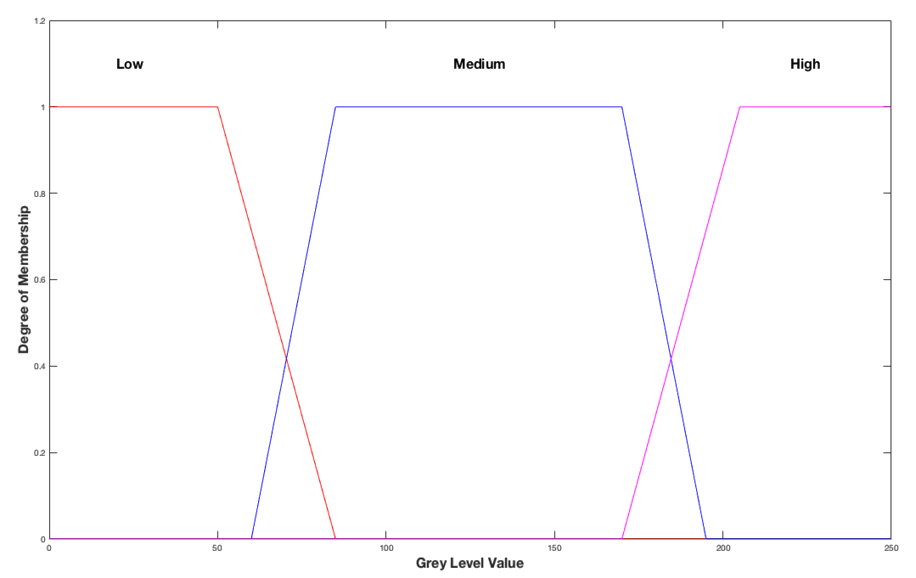
\includegraphics[scale=0.4]{Chapter2/hybrid-img/3_traps.png}
  \caption{3 trapezium-shaped membership sets}
  \label{fig:3-trapeziums}
\end{figure}

\subsection{Fuzzy Entropy choices}

\textbf{Chosen algorithms:}
\begin{itemize}
  \item Non-Probability Entropy
  \item Hybrid Entropy
\end{itemize}

Given the simplistic nature of Non-Probabilistic entropy, this was one of the chosen Fuzzy Entropy algorithms to be implemented in the project.

Hybrid entropy was chosen for implementation in this project due to it's hybrid nature (implementing both Probabilistic and Possibilistic uncertainty) and for it's simplification nature - in the absence of fuzziness, then $E_0$ and $E_1$ reduce to $p_0$ and $p_1$ respectively, therefore classical Shannon entropy. This is especially useful in image processing, and other such areas which deal with a lot of noise.

\textbf{Discarded algorithms:}
\begin{itemize}
  \item Fuzzy Shannon Entropy
\end{itemize}

The initial plan was to implement this algorithm in the project - however after further investigation which revealed that Fuzzy Shannon Entropy does not model Probabilistic uncertainty - it was decided that this algorithm was to be excluded.

\subsection{Image Alignment choice}

\textbf{Image Alignment choice:}
\begin{itemize}
    \item \Gls{Congealing}
\end{itemize}

As this project will be working with mammograms, something with little variation nor inconsistency, \Gls{Congealing} is the perfect, light-weight image alignment algorithm to which to build upon, especially as the demonstration code available for research has an entropy implementation already developed.

\textbf{Discarded Image Alignment choice:}
\begin{itemize}
    \item Least squares \gls{Congealing}
    \item Joint Alignment of Complex Images
\end{itemize}

Least squares \gls{Congealing} algorithm was disregarded for this project due to the preference to focus upon entropy-based alignment algorithms and the computational costs that the authors themselves regard to be a drawback of their algorithm.

The Complex implementation of \Gls{Congealing} was quickly identified as overly complex for this project. The original \Gls{Congealing} algorithm was more appropriate for grey-scale mammograms, with a consistent canonical pose.



\section{Implementation tools}

\subsection{MATLAB}
\label{ssec:matlab}

\subsection{Version Control}
